\capitulo{4}{Técnicas y herramientas}

\section{Gestión de proyectos - Scrum}
Scrum es un marco de trabajo ágil utilizado para la gestión de proyectos software. Este marco de trabajo está basado en \textit{sprints} de entre una y cuatro semanas de duración. En estas iteraciones se genera un incremento de software que sea potencialmente entregable ~\cite{scrum:latex}.

En este proyecto, se ha utilizado esta metodología pero algo adaptada, dado que es un proyecto individual. Las reuniones retrospectivas propias de Scrum, se tenían con los tutores del proyecto cada dos semanas. En estas reuniones se evaluaban las tareas realizadas hasta la fecha y se establecían unos nuevos objetivos para el próximo sprint. Estas tareas, fueron detalladas en el apartado de \textit{Issues} en la plataforma GitHub.  

\section{Herramienta de control de versiones - Git}
Git es un sistema de control de versiones distribuido. Los desarrolladores dispondrán de copias completas del repositorio permitiendo de esta manera trabajar sin conexión o de forma remota con facilidad ~\cite{git:latex}.

Los desarrolladores deben hacer \textit{commit} para almacenar su trabajo de manera local y posteriormente se sincronizará la copia del repositorio con la del servidor. Esto nos proporciona gran facilidad para tener un control total sobre los cambios realizados en nuestro código.

En el proyecto, se ha trabajado con esta herramienta mediante el uso de la terminal \textit{Git Bash}. Además, se realizaban actualizaciones periódicas al repositorio de GitHub para, de esta manera, que permaneciesen tanto el repositorio local como el repositorio remoto actualizados.

\section{Repositorio remoto - GitHub}
GitHub es una herramienta web que permite el alojamiento de proyectos en repositorios remotos. Además, utiliza Git para el control de versiones lo cual es tremendamente útil para tener un control de los cambios realizados a lo largo del ciclo de vida del proyecto. 

Los repositorios son los lugares donde se almacena el código del proyecto en la nube. Estos pueden ser públicos o privados en función de la decisión del usuario ~\cite{github:latex}.

En este proyecto se ha decidido utilizar esta herramienta debido a la facilidad de uso y las enormes ventajas que nos proporciona. Además es una herramienta sobre la cual es fundamental tener amplios conocimientos debido a la importancia que tiene en el mundo laboral.

El enlace al repositorio de GitHub utilizado en este proyecto, es el siguiente: \href{https://github.com/miguelUbierna/DeltaOffers}{https://github.com/miguelUbierna/DeltaOffers}
\section{Entorno de desarrollo}

\subsection{Visual Studio Code}
Visual Studio Code es un editor de código desarrollado por Microsoft disponible para diferentes Sistemas Operativos ~\cite{vscode:latex}. Ofrece numerosas funcionalidades como autocompletado inteligente, refactorización o depuración de código.

Este editor de código ha sido el utilizado para realizar la aplicación en la que se realiza el \textit{web scraping} y se actualiza la base de datos. El lenguaje de programación utilizado en esta herramienta ha sido Python, para ello, Visual Studio Code nos proporciona una extensión de Python para facilitarnos el desarrollo en este lenguaje.

\subsection{Visual Studio Community}
Microsoft Visual Studio es un entorno de desarrollo disponible para diferentes sistemas operativos. Este nos permite programar en múltiples lenguajes y entornos de desarrollo.

Este entorno ha sido utilizado para realizar la aplicación web del proyecto mediante la utilización del \textit{framework} ASP .NET Core MVC. Se eligió este entorno de desarrollo por la facilidad de creación de aplicaciones web con el mismo ~\cite{vscommunity:latex}.

\section{Web scraping}
El \textit{web scraping} es la técnica utilizada para la extracción de información y datos de las páginas web ~\cite{webscrapingwiki:latex}. Los usuarios que interactuamos con las aplicaciones web, podemos ver la información que aparece en las mismas. Sin embargo, los datos e información en la mayoría de páginas webs, no están disponibles para su descarga. Es ahí donde el \textit{web scraping} juega un papel importante ~\cite{webscraping:latex}.

En el caso del proyecto, este proceso de raspado de la web ha sido realizado mediante código, concretamente utilizando el lenguaje de programación Python.

Para ello, hemos tenido que ayudarnos de algunas librerías existentes que están dedicadas a realizar este tipo de técnicas.

En este proyecto en concreto, hemos realizado \textit{web scraping} de las webs de las universidades públicas de Castilla y León para obtener los datos sobre sus convocatorias.

A continuación, se van a comentar las bibliotecas que nos han sido de ayuda para este proceso.

\subsection{Requests}
Requests es una biblioteca disponible para utilizar desde el lenguaje de programación Python que nos permite realizar solicitudes HTTP de manera muy sencilla. Esta herramienta se utiliza para obtener el contenido de páginas web o para hacer peticiones a APIs ~\cite{requests:latex}.

Esta biblioteca ha sido utilizada para hacer las peticiones HTTP a las webs de la Universidad de Burgos y la Universidad de León. 

Para un uso correcto de la misma, en primer lugar hacíamos una petición y verificábamos que el código de estado devuelto era correcto. Posteriormente, accedíamos el texto que devolvía esa petición, el cual era el código HTML de la página web solicitada. 

Una vez que tenemos el código HTML en nuestro programa, finalizaba el uso de esta biblioteca y comenzábamos a utilizar otras más específicas para la extracción de datos.

\subsection{Beautiful Soup}
Beautiful Soup es una biblioteca de Python utilizada para la extracción de datos de los documentos HTML Y XML ~\cite{soup:latex}. Para una utilización exitosa de esta herramienta, es necesario indicar cual es el \textit{parser}. Este va a ser el encargado de transformar los documentos HTML en un árbol de objetos. El parser utilizado en este proyecto ha sido \textit{lxml}, este es uno de los más comúnmente utilizados .

Un paso previo antes de utilizar esta biblioteca, es encontrar y localizar los elementos de interés. Para ello, en este proyecto se realizó un proceso de análisis previo en el que se inspeccionó el código HTML de las webs a las que se quería hacer el raspado.

Por último, se accederán a los elementos deseados que han sido analizados previamente. Este acceso a elementos se puede realizar a través de las etiquetas, clases, identificadores, atributos o texto. En el caso de este proyecto, en la mayoría de ocasiones se ha realizado el acceso a elementos mediante sus clases, pero en ocasiones dado que había varias clases del mismo nombre, se ha cambiado esta estrategia ~\cite{beautifulsoup:latex}.

\begin{figure}[H]
    \centering
    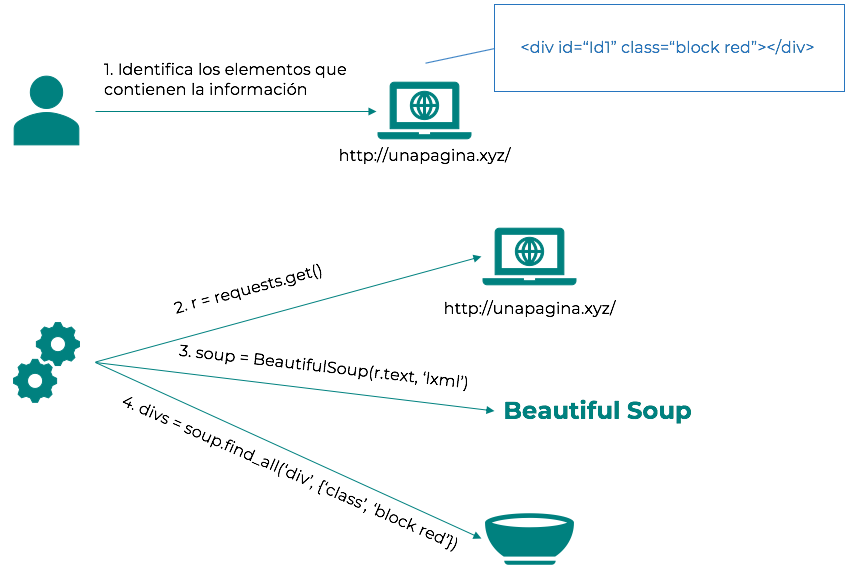
\includegraphics[width=0.75\linewidth]{DocumentacionTFG//img/WebScrapingPython.png}
    \caption{Pasos Web Scraping con Beautiful Soup y Requests}
    \label{fig:enter-label}
\end{figure}

\subsection{Selenium}
Selenium es una herramienta que permite la automatización de navegadores web. Principalmente, es utilizada para la grabación, edición o depuración de pruebas en aplicaciones web pero también es posible utilizarla para la realización de \textit{web scraping} ~\cite{selenium:latex}.

Esta herramienta está disponible para múltiples lenguajes de programación, en este caso se ha utilizado con Python. Para que Selenium funcione correctamente, los usuarios necesitan dos requisitos previos:

\begin{itemize}
    \item \textbf{Navegador Web:} Se necesita que el usuario tenga un navegador web instalado en el sistema. En el proyecto, el navegador utilizado fue Firefox dado que esta herramienta fue utilizada para hacer \textit{web scraping} de la UVA cuya web recomendaba que fuese abierta con dicho navegador.
    \item \textbf{Driver:} Es el encargado de manejar las peticiones del usuario y el que nos permite interactuar con las páginas web.
\end{itemize}

Se optó por la utilización de esta herramienta dado que el contenido de la página web de la Universidad de Valladolid se cargaba mediante JavaScript dinámico. Por esta razón, pese a tener un mayor dominio de la herramienta Beautiful Soup, se realizó el \textit{web scraping} de la web de la universidad mencionada con Selenium.

\section{MySQL}
MySQL es un sistema de gestión de bases de datos de código abierto desarrollado por Oracle el cual utiliza el lenguaje SQL ~\cite{mysql:latex}.

Se decidió utilizar MySQL como herramienta de gestión de bases de datos debido a su rendimiento y fiabilidad de uso. Además, gracias a que la base de datos es relacional, tendremos una estructura del dato mucho más definida.

Quizás, el acceso a datos sea más rápido y de menor coste en cuanto a rendimiento mediante la utilización de una base de datos no relacional, pero, dado que la aplicación realizada no requiere de una carga de datos masiva, esta diferencia en cuanto a tiempos es despreciable.

En las primeras etapas del proyecto, instalé MySQL Server en mi máquina local. Esto me permitió realizar las pruebas de carga de datos en la base de datos utilizada. Posteriormente, una vez que tenía la aplicación preparada para el despliegue, decidí migrar la base de datos de mi entorno local a un servidor MySQL Azure.


\section{ASP.NET Core MVC}
ASP.NET Core MVC es un \textit{framework} utilizado para construir aplicaciones web y API mediante la utilización del patrón de diseño Modelo-Vista-Controlador ~\cite{.net:latex}. El lenguaje de programación utilizado en este \textit{framework} es principalmente C\# aunque también contiene soporte para HTML, CSS y Javascript.

Las principales ventajas que nos proporciona este \textit{framework} son las siguientes:

\begin{itemize}
    \item Framework Multiplataforma
    \item Proporciona gran rendimiento y escalabilidad
    \item Modular
    \item Soporte para la inyección de dependencias
\end{itemize}

Esta herramienta ha sido la utilizada para la aplicación web del proyecto y se han seguido con ella la siguientes pasos para el desarrollo de la misma:


\begin{itemize}
    \item En primer lugar, se definían los modelos y el contexto en función de la base de datos MySQL diseñada previamente.
    \item Posteriormente, se realizaba en acceso a datos e implementación de la lógica desde los controladores. Una vez la lógica estaba implementada, se pasaban los datos a la vista.
    \item La vista será la encargada de mostrar los datos y la interacción con el usuario final.
\end{itemize}

Una vez entendido cómo funciona este \textit{framework}, vamos a mencionar cuales han sido las extensiones utilizadas en la aplicación.

\subsection{X.PagedList.Mvc.Core}
Esta librería permite aplicar paginación a listas en aplicaciones web ASP.NET Core MVC ~\cite{pagedlist:latex}.
Esto mejora enormemente la usabilidad de la aplicación dado que las convocatorias del PDI Y PAS estarán divididas en distintas páginas permitiendo navegar fácilmente entre ellas.


\subsection{Pomelo.EntityFrameworkCore.MySql}
Esta librería es la que nos ha permitido conectar de manera eficiente nuestra aplicación en .NET con la base de datos MySQL.

Pomelo.EntityFrameworkCore.MySql es un proveedor de Entity Framework Core construido sobre MySqlConnector que permite el uso de Entity Framework Core ORM con MySQL. Esto nos ha permitido la interacción con la base de datos mediante objetos en vez de utilizar consultas SQL ~\cite{pomelomysql:latex}. 

\subsection{MailKit}
Esta biblioteca de .NET tiene como propósito el envío, recepción y manipulación de correos electrónicos y suele ser frecuentemente usada en aplicaciones web que utilizan la automatización de correos electrónicos ~\cite{mailkit:latex}.

En el proyecto realizado, ha sido utilizada para el envío de correos mediante la utilización del protocolo SMTP ~\cite{smtp:latex}. El protocolo simple de transferencia de correo, es un protocolo TCP/IP utilizado para el envío y la recepción de correos electrónicos.

Esta biblioteca y este protocolo han sido utilizados para la implementación de un sistema de avisos basado en correo electrónico.

\section{GitHub Actions}
Esta herramienta, permite la personalización, automatización y ejecución de flujos de trabajo en los repositorios de GitHub.

Este es un servicio de integración continua y entrega continua que permite la automatización de compilaciones, pruebas y despliegue.

Estos flujos de trabajo aparecen en el directorio \textit{.github/workflows} dentro de un repositorio de GitHub. Este directorio contendrá uno o varios flujos de trabajo los cuales realizarán unas tareas ~\cite{githubactions:latex}.

En el caso del proyecto, se ha utilizado esta herramienta para la realización de actualizaciones periódicas a la base de datos. Para ello, se han definido dos tareas programadas que ejecutarán dos archivos Python en función de la fecha y hora definida en el \textit{cron}. Esta tarea programada al igual que el resto de flujos de trabajo, ha sido definida en un archivo de extensión \textit{.yml}.

La utilización de GitHub Actions ha sido de tremenda ayuda a la hora del despliegue del proyecto dado que ha permitido la ejecución de tareas programadas sobre el código sin necesidad de realizar estas tareas de manera local o con un coste mayor.

\section{Microsoft Azure}

Azure es una plataforma de Microsoft que ofrece servicios en la nube, con ella, se pueden crear, probar y desplegar aplicaciones y servicios mediante la utilización de los servidores proporcionados por Microsoft. Esta plataforma supone una enorme ventaja a la hora de tener tus proyectos en la nube sin que sea necesario tener una infraestructura física propia ~\cite{azure:latex}.

Los servicios Azure utilizados en este proyecto, han sido dos:

\begin{itemize}
    \item \textbf{Servidor de Azure Database para MySQL ~\cite{azuremysql:latex}:} Proporciona MySQL totalmente administrado de gran rentabilidad, seguridad y flexibilidad. 
    Este servidor se ha utilizado para desplegar la base de datos MySQL utilizada en el proyecto con las convocatorias correspondientes del PDI Y PAS.
     \item \textbf{Azure App Services ~\cite{azureappservices:latex}:} Este es un servicio basado en HTTP que permite hospedar aplicaciones web en la nube. Este servicio permitió desplegar la aplicación con facilidad, de manera segura y sin tener preocupación por la infraestructura del sistema. Otra ventaja de este servicio, es su compatibilidad con diferentes \textit{frameworks} y lenguajes de programación. 
     
     Por otro lado, Azure App Service permite la integración con otros servicios de Azure. Esto nos permitió realizar la conexión del servidor  MySQL con el que se desplegó la base de datos de manera sencilla.
     

\end{itemize}


\section{Diseño adaptativo}

El diseño adaptativo es una rama del diseño web que tiene como objetivo la adaptación de las ventanas de las páginas web a cualquier tipo de dispositivo independientemente del ancho de pantalla ~\cite{adaptativo:latex}. Esto quiere decir que una página web adaptativa, debe poder utilizarse en ordenadores, \textit{tablets} o \textit{smartphones}. 

Para conseguir el objetivo de que la página web sea adaptativa, se han utilizado las \textit{media queries} ~\cite{mediaqueries:latex}, estas permiten la aplicación de estilos CSS según un ancho determinado de la pantalla.

Para ello, se iban indicando los correspondientes anchos de pantalla e interiormente se van definiendo los nuevos estilos CSS. A continuación se muestra en ejemplo de una de las \textit{medias queries} realizadas en el proyecto.

\begin{figure}[H]
    \centering
    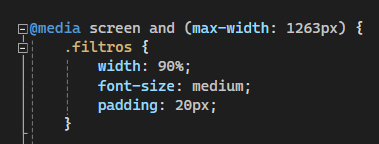
\includegraphics[width=0.6\linewidth]{DocumentacionTFG//img/MediaQueries.PNG}
    \caption{Aplicación media queries en CSS}
\end{figure}

Finalmente, se consiguió que nuestra web tuviese un diseño adaptativo. A continuación, se va a mostrar como quedaría una ventana de la aplicación desarrollada para distintos dispositivos.

\begin{figure}[H]
    \centering
    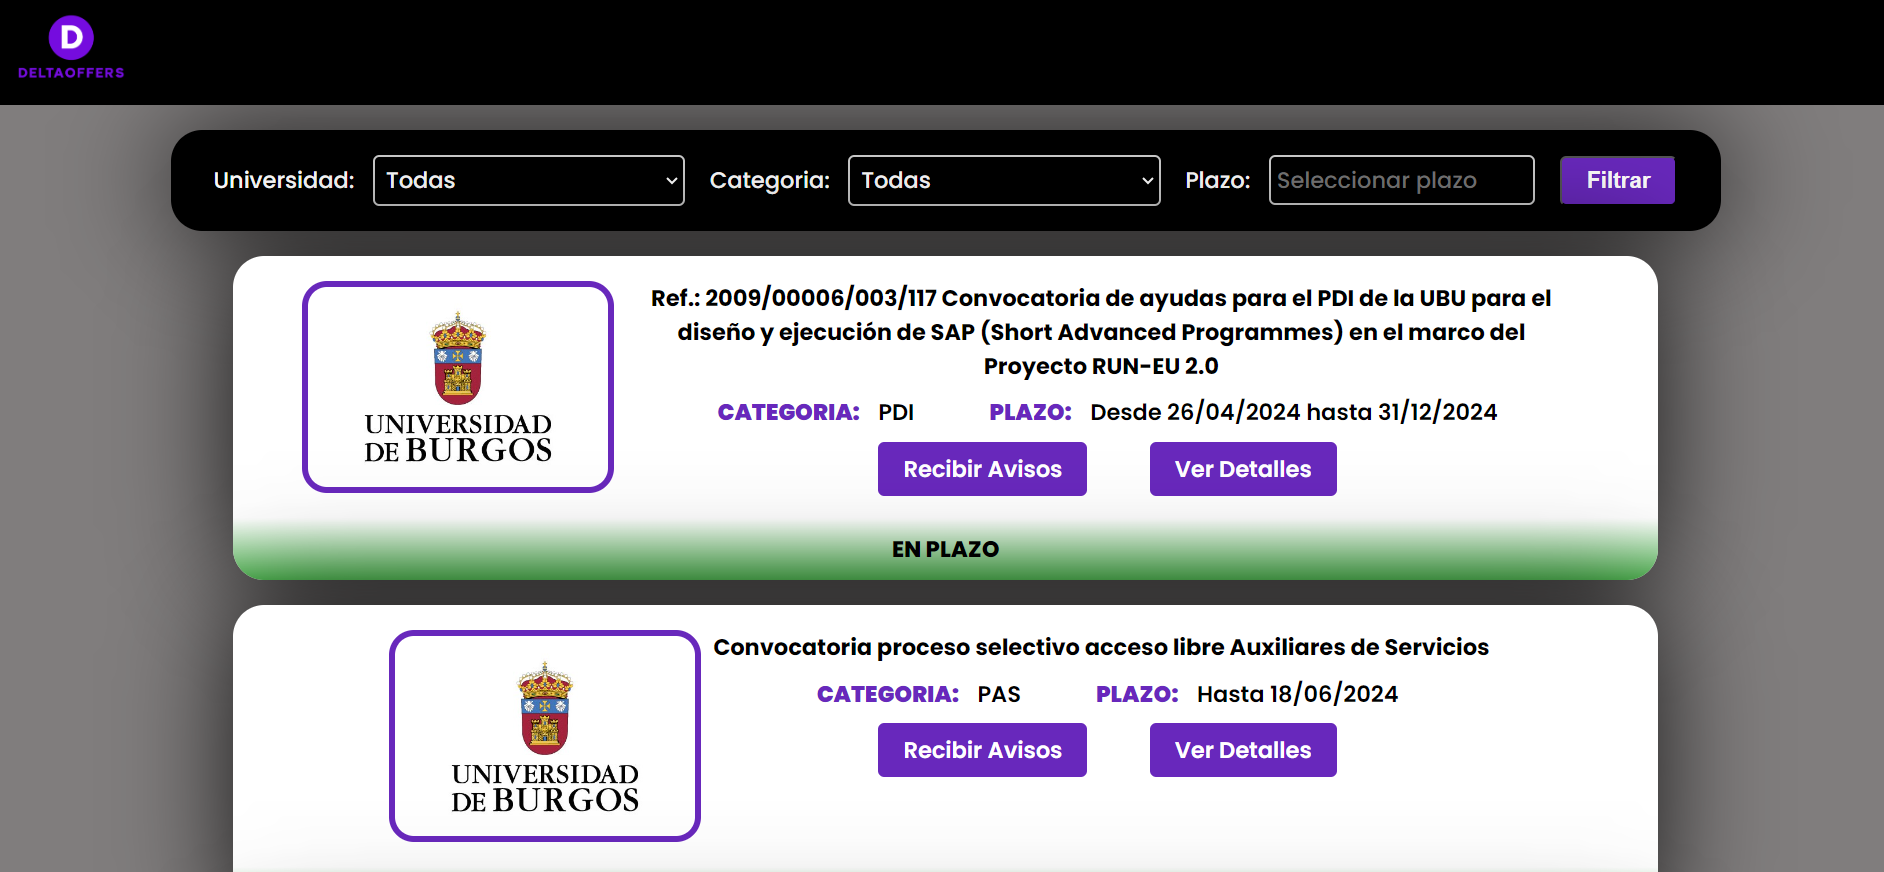
\includegraphics[width=0.8\linewidth]{DocumentacionTFG//img/VisualizacionConvocatorias.PNG}
    \caption{Visualización convocatorias en pantalla de ordenador}
\end{figure}

\begin{figure}[H]
    \centering
    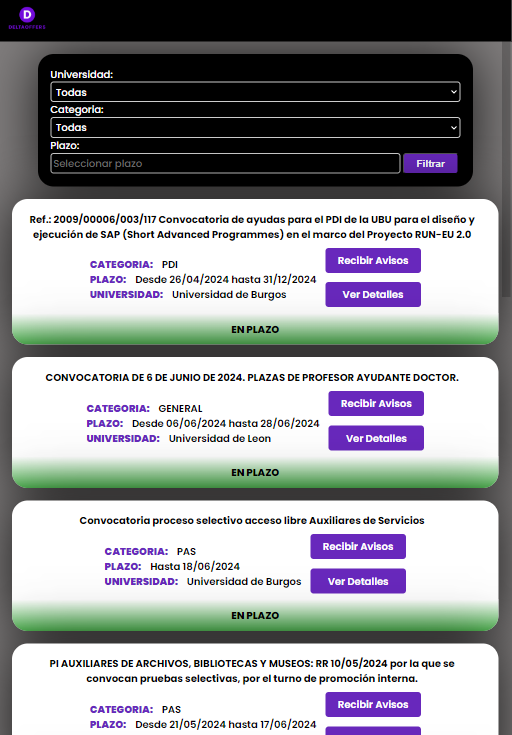
\includegraphics[width=0.8\linewidth]{DocumentacionTFG//img/VisualizacionPantallaTablet.PNG}
    \caption{Visualización Convocatorias Pantalla Tablet}
\end{figure}

\begin{figure}[H]
    \centering
    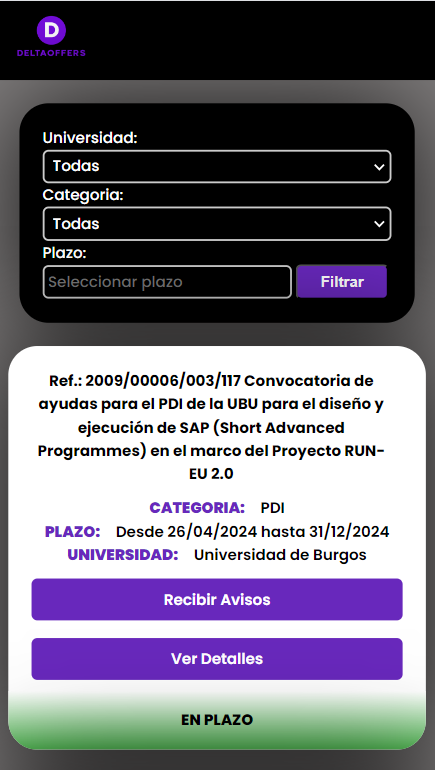
\includegraphics[width=0.5\linewidth]{DocumentacionTFG//img/VisualizacionPantallaSmartphone.PNG}
    \caption{Visualización Convocatorias Pantalla Smartphone}
\end{figure}

\section{Testing}
La implementación de test unitarios, fue realizada en la aplicación de \textit{web scraping}. De esta manera se comprobaban si las convocatorias y campos obtenidos eran los correctos.

Las herramientas de \textit{testing} utilizadas han sido las siguientes:

\begin{itemize}
    \item \textbf{Unit Test: ~\cite{unittest:latex}} Esta es una biblioteca utilizada en Python para la creación y ejecución pruebas de manera automática. Unit Test permite la realización de pruebas unitarias de una manera organizada y con gran variedad de métodos de aserción. La utilización de esta herramienta aplicada a programas en Python es clave para que los desarrollos realizados sean de calidad.
    \item \textbf{MagicMock:} Esta biblioteca de pruebas utilizada en Python, permite el reemplazamiento de partes del sistema a cambio de objetos simulados. Esto ayuda a reducir la cantidad de código auxiliar que muchas veces podemos encontrar en los entornos de pruebas. De esta manera evitamos la utilización de los objetos para la realización de test unitarios de manera directa.
\end{itemize}


\section{Guía de estilos de código}
Para asegurarnos de disponer de un código bien estructurado y de calidad, se decidió utilizar la guía de estilos PEP 8. Esta guía de estilos fue aplicada gracias a la biblioteca Autopep8 proporcionada y a su fácil integración con el entorno de desarrollo Visual Studio Code.  

Esta guía define conceptos como la longitud de las líneas, la indentación, las líneas en blanco y la guía de importación de otros paquetes ~\cite{pep8:latex}.

\section{Documentación}
\LaTeX \quad ha sido la herramienta utilizada para la documentación del proyecto. Esta, permite la creación de textos orientados a documentos escritos de gran calidad tipográfica ~\cite{latex:latex}.

Esta herramienta suele ser utilizada para la redacción de libros y artículos científicos, esto se debe a la gran facilidad que presenta para la escritura de fórmulas y expresiones matemáticas. Quizás no se utilice todo lo que debería dado que comparada con otros procesadores de texto, esta tiene una curva de aprendizaje alta.


\section{Lenguajes de Programación}
En esta sección se van a comentar los lenguajes de programación utilizados para el desarrollo del proyecto y la finalidad con la que se ha utilizado cada uno de ellos.

\begin{itemize}
    \item \textbf{Python:} Este lenguaje ha sido utilizado para la realización del \textit{web scraping}. Además, una vez recopilados los datos, se realizó un tratamiento y limpieza de los mismos.
    
    Finalmente, este lenguaje también fue utilizado para la actualización de la base de datos del sistema.
    \item \textbf{CSS:} Lenguaje que se encarga de la apariencia y diseño de la página web realizada. Otro aspecto importante a considerar, serían las \textit{media queries} aplicadas para la realización de la aplicación con diseño adaptativo.
    \item \textbf{C\#:} Utilizado para el desarrollo de la aplicación web en ASP .NET Core MVC dentro de los modelos, los controladores e incluso en las vistas de manera embebida.
    \item \textbf{HTML:} Lenguaje utilizado para mostrar la estructura y contenido de la página web.
    \item \textbf{JavaScript:} Utilizado para aportar funcionalidades en el lado del cliente. Principalmente utilizado para validaciones, formularios y animaciones en la aplicación web.
\end{itemize}

GitHub proporciona una gráfica en la que se indica qué porcentaje de cada lenguaje de programación hay en mi repositorio. La gráfica es la siguiente:

\begin{figure}[H]
    \centering
    \includegraphics[width=0.75\linewidth]{DocumentacionTFG//img/PorcentajeLenguajesProgramación.PNG}
    \caption{Porcentaje de cada lenguaje de programación en el proyecto}
    \label{fig:enter-label}
\end{figure}